\documentclass[12pt]{article}
	
%______________________PREAMBULO_________________________

%----------------------Paquetes--------------------------
\usepackage{amsmath,amssymb,amsfonts,latexsym,cancel} % Paquetes de símbolos adicionales.
\usepackage[spanish,es-tabla]{babel} % Idioma español
\usepackage[utf8]{inputenc} % Paquete que nos permite usar los acentos y otros símbolos, directamente del teclado.
\usepackage[T1]{fontenc} % Cambia el tipo de letra
\usepackage{times} % Tipo de letra Times New Roman
\usepackage{graphicx} % Paquete para el manejo de gráficos y figuras en el documento.
\usepackage{geometry} % Permite el manejo de los margenes
\usepackage{fancyhdr} % Permite colocar y manejar el encabezado
\usepackage[breaklinks,colorlinks=true,linkcolor=black,citecolor=blue, urlcolor=blue]{hyperref} % Crea hipervinculo entre secciones y el indice
\usepackage{pstricks}
\usepackage{multicol}
%\usepackage{mathpazo} %fuente palatino
%\usepackage{xcolor}
%\usepackage[shortlabels]{enumitem}
%-------------Paquetes para el formato de las citas-------
%\usepackage[hyphens]{url}
%\usepackage{float}
%\usepackage{cite}
%\usepackage{wrapfig}

%-----------------------------ayuda de paquetes--------------------

\spanishdecimal{.}

%------------------------Margenes----------------------------

\newgeometry{bottom = 2.5 cm, top = 2.5 cm, left = 2 cm, right = 2 cm} % Modifica el margen {Abajo, Arriba, Izquierda, Derecha

%----------------------------Interlineado----------------------------------

%\doublespacing
%\onehalfspace
%\singlespace
%\spacing{1.5} % Permite personalisar a gusto
%\setlength{\parskip}{2cm} % Es el espacio entre parrafos

%-----------------------------Sangria---------------------------------------

\setlength{\parindent}{0 cm} % Manipula la sangria

%---------------------Portada------------------

%\title{
%\begin{figure}[h!]
		
%	\centering
%	
\includegraphics[width=\linewidth]{Nom_UAdeC_FCFM.png}  			
			
%\end{figure}
%\huge \textbf{LABORATORIO DE FISICA 3}\\\LARGE TITULO PRACTICA\\}
%\author{ \Large \textbf{Profesor:}\\
%\Large \textbf{Alumno:} Oscar Joel Castro Contreras}
%\date{\today}

%--------------Encabezado y pie de pagina--------------------

\pagestyle{fancy}%Coloca el encabezado en el documento
\lhead[]{Métodos numéricos}%Encabezado izquierda
\rhead[]{Oscar Joel Castro Contreras}%Encabesado derecha
%\chead[]{}%Encabesado central
\renewcommand{\headrulewidth}{0.08 pt}%Coloca linea al pie de pagina

%\lfoot[]{PI}%Pie de pagina izquerdo
%\rfoot[]{PD}%Pie de pagina derecho
\cfoot[]{\thepage}%Pie de pagina central
\renewcommand{\footrulewidth}{0.08 pt}%Coloca linea al pie de pagina

%-----------------------------------------------------------------------------

	\begin{document}
		
		\begin{titlepage}
		
			\centering
			{\bfseries
			\begin{figure}[h!]
				\centering
				
\includegraphics[width=\linewidth]{Nom_UAdeC_FCFM.png} 				
			\end{figure}
			\par}
			\vspace{2cm}
			{\scshape\LARGE Métodos numéricos \par}
			\vspace{3cm}
			{\scshape\Huge \textbf{Método de Newton Raphson} \par}
			\vfill
			{\LARGE \textbf{Profesora:} Maria Guadalupe Godina Cubillo \par}
			\vspace{3cm}
			{\LARGE \textbf{Alumno:} Oscar Joel Castro Contreras \par}
			\vfill
			{\Large \today \par}
			\thispagestyle{empty}
			%\thispagestyle{fancy}
			
		\end{titlepage}
	
		\newpage

		\begin{abstract}
			\noindent En este reporte explico un poco de los métodos que existen para encontrar las raíces de cualquier 
			polinomio o función que tenga raíces, y en específico explico, qué es, en que consiste y cuales son las 
			limitaciones del método de Newton Raphson para encontrar raíces.
		\end{abstract}

		\textbf{Palabras clave:} Raíces, Newton Raphson, Tangente, Derivada, Maximo, Mínimo.

		\section*{\centering Introducción}\label{sec:Introducción}
			Los polinomios son uno de los conceptos más importantes en álgebra y son fundamentales en 
			matemáticas y ciencia en general. Determinar las raíces de un polinomio es uno de los problemas 
			más antiguos en matemáticas.\\
			Puesto que las ecuaciones polinomiales aparecen en un amplio rango de áreas de la ciencia, desde 
			química y física básica hasta economía, el problema de determinar raíces de polinomios es, con 
			frecuencia, un paso obligado en la resolución de problemas.\cite{bib:item1}\\
			La razón principal para resolver ecuaciones no lineales por medio de métodos computacionales es 
			que algunas ecuaciones carecen de solución exacta, excepto por unas pocas. Por lo que existen 
			métodos numéricos diseñados para obtener las raíces, aunque cada uno tiene sus propias 
			limitaciones y defectos. Algunos métodos se muestran en la tabla \ref{tab:1}\cite{bib:item2}\\
			\begin{table}[h!]
				\centering
				\begin{tabular}{|c|c|}
					\hline
					\multicolumn{2}{|c|}{\textbf{Métodos numéricos para obtener raíces}}\\
					\hline
					\textbf{Nombre} & \textbf{Características} \\\hline
					Bisección & Aplicable a funciones no analiticas \\\hline
					Regla falsa & Convergencia lenta en un intervalo grande \\\hline								
					Método de Newton & Rápido, se nesecita calcular derivada \\\hline
					Método de secante & Rápido, no se requiera calcular derivada \\\hline
					Sustitución sucesiva & Puede no converger \\\hline
				\end{tabular}
				\caption{Métodos numéricos para obtener raíces \cite{bib:item2}}
				\label{tab:1}
			\end{table}\\
			En general, no es posible determinar los ceros de una función, es decir, valores $ x^* $ tal que $f(x^*) = 0 $, 
			en un número finito de pasos. Tenemos que usar métodos de aproximación. Los métodos son 
			usualmente iterativos y tienen la forma: Iniciando con una aproximación inicial $ x_0 $ (o un intervalo $ [a,b] $) , 
			se calculan aproximaciones sucesivas $ x_1,x_2,... $ y elegimos $ x_n $ como aproximación de $ x^* $ cuando se cumpla un 
			criterio de parada dado. A los ceros de un polinomio se les conoce también como raíces.\\
			\textbf{El método de Newton Raphson:}\\
			Utiliza las rectas tangentes que se evalúan analíticamente. El método de Newton se puede aplicar 
			al dominio complejo para hallar raíces complejas. También se puede extender a las ecuaciones no 
			lineales simultaneas. \cite{bib:item3} \\
			La fórmula de Newton-Raphson sea la más ampliamente utilizada. Si el valor inicial para la raíz es 
			$ a $, entonces se puede trazar una tangente desde el punto $ (a,f(a)) $ . Por lo común, el punto donde 
			esta tangente cruza al eje x representa una aproximación mejorada de la raíz. El método de Newton 
			Raphson se deduce a partir de esta interpretación geométrica (un método alternativo basado en la 
			serie de Taylor). Se tiene que la primera derivada de la función es equivalente a la pendiente: 
			$$ f'(x) = \frac{f(x)-0}{x-x_1} $$ que se arregla para obtener $$ x_1 = x - \frac{f(x)}{f'(x)} $$ 
			la cual se conoce como fórmula de Newton Raphson. \cite{bib:item4}

		\section*{\centering Metodología}\label{sec:Metodologia}
			El método a diferencia de bisección y regla falsa solo toma un valor inicial $ a $ estimado, de donde 
			esta la raíz de la función y con la primera derivada de la función se traza un recta tangente que cruce 
			por el punto $ (a,f(a)) $, esta recta tangente a la función cruza por el eje $ x $ en un cierto punto, 
			este punto es una aproximación a la raíz. Entonces el método se basa en que la primera derivada de 
			la función es una aproximación a la pendiente de la recta por lo que tenemos $$ f'(x) = \frac{f(a)-0}{a-x} $$ 
			si dejamos $ x $ $$ x = a - \frac{f(a)}{f'(a)} $$, esta x calculada ahora lo cambio por nuestro valor 
			inicial $ a = x $ y así vamos iterando las veces necesarias hasta encontrar la mejor aproximación a la 
			raíz de la función. Si la función tiene mas de una raíz, el método encuentra la raíz que se encuentra 
			más cerca al valor inicial dado. \\
			El criterio para parar las iteraciones es el mismo que bisección y ragla falsa, está dado por el número de cifras 
			significativas que queramos, de aquí obtenemos una tolerancia, la cual en cada interacción se 
			compara con el error relativo y absoluto, si uno de los errores es menor o igual a la tolerancia, 
			detener las interacciones.\\
			El programa se basa mucho en lo explicado antes, en esta parte de mi programa se obtiene la 
			derivada de la función $ (der) $, se evalúan el valor inicial $ (a) $, en la derivada $ (fder) $ y la función $ (fa) $ 
			y por ultimo se calcula el punto por el que se cursa en eje $ x $ $ (r) $, esta parte es la mas 
			importante del programa, ya que de aquí se obtiene la aproximación a la raíz.
			\begin{center}
				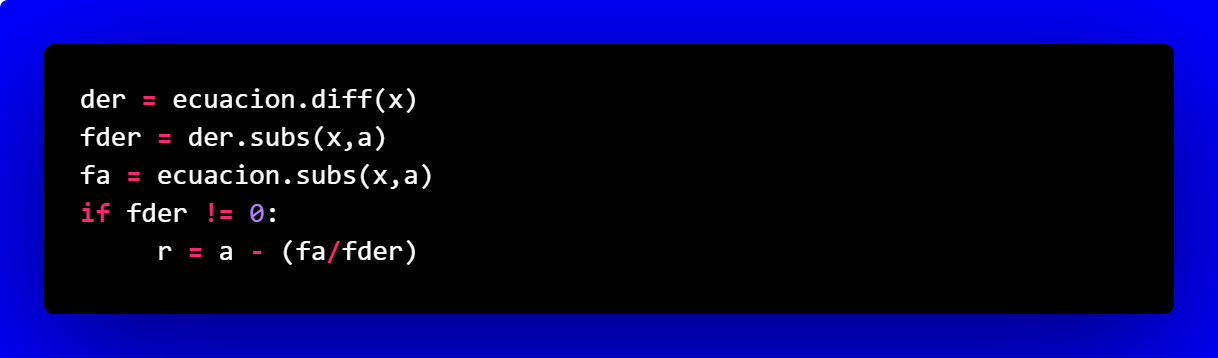
\includegraphics[width=\linewidth]{Figura 1.png} 				
			\end{center}
		
		\section*{\centering Resultado}\label{sec:Resultado}
			Si tomamos el polinomio $ x^3-2x^2-1 $ y damos el punto $ x = 1 $. Hacemos 
			la evaluación para obtener la raíz con 5 cifras significativas, el programa nos arroja
			\begin{multicols}{2}
				\begin{center}
					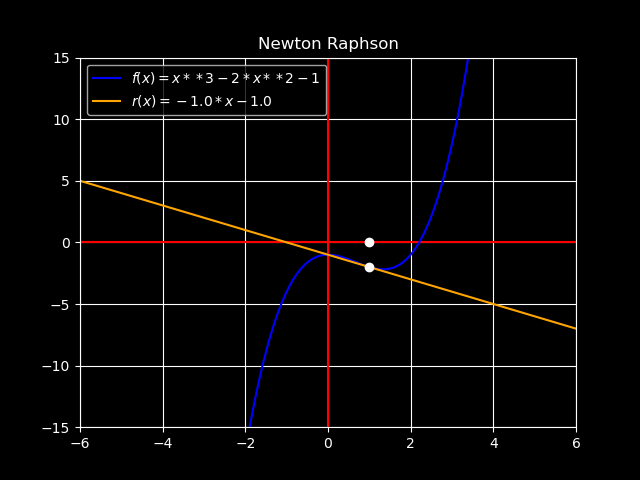
\includegraphics[width=\linewidth]{Grafica 1.png}
					Grafica 1: Recta Tangente de la funcion que cruza \columnbreak $ x^3-2x^2-1 $ en $ x = 1 $.\\
					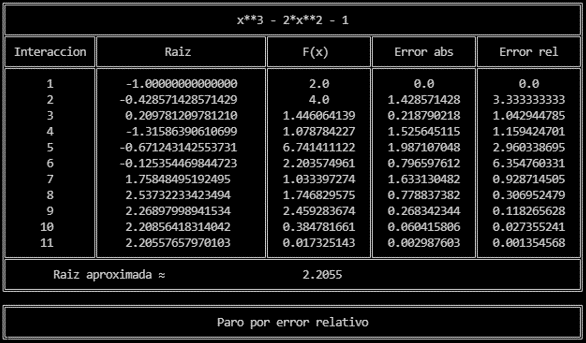
\includegraphics[width=\linewidth]{Tabla 1.png}
					Tabla 2: Iteraciones a la aproximación de la raíz de la función $ x^3-2x^2-1 $.
				\end{center}
			\end{multicols}
			Observamos que la aproximación a la raíz es $ 2.2055 $, con 11 iteraciones. El criterio de paro fue 
			por el error relativo.
		\section*{\centering Observación}\label{sec:Observacion}
			El método tiene algunas limitaciones, una de ellas es que en algunos casos la derivada de la función 
			caerá en los máximos o a un mínimo de la función, cuando ocurre esto la recta deja de cruzar por el 
			eje $ x $, por lo que en estos casos el método se parar y se le debe de pedir al usuario que coloque 
			un valor inicial un más cercano a la raíz. Otra de las limitaciones es cuando la función no tiene raíces 
			reales, cuando se queda en un bucle donde la función tiene un valor mínimo o cuando se colocó un 
			valor inicial muy lejano a la raíz y en vez de que el método converger este diverge, en estos casos el 
			método nunca deja de iterar, por lo que se le debe de dar un paro a una cierta cantidad de iteraciones.

		\section*{\centering Conclusión}\label{sec:Conclusion}
			En conclusión, el método de Newton Raphson, toma un valor inicial $ a $ y con la ayuda de la derivada de la 
			función y la pendiente de la recta tangente que cruza por el punto $ (a,f(a)) $ 
			se obtiene una formula con la que se puede calcular, por donde cruza la recta tangente el eje $ x $, 
			e sustituir el valor inicial por el nuevo valor encontrado $ a = x $ y evaluar de nuevo la función, pero 
			ahora con el nuevo valor y así ir iterando hasta llegar a la raíz de la función. Las limitaciones del 
			método son, cuando la derivada de la función cae en un máximo o un mínimo de la función, cuando 
			la función no tiene raíces reales o cuando la recta se queda en un bucle donde hay un mínimo de la 
			función y cuando se coloca un valor inicial muy lejos de la raíz donde puede que, en vez de 
			converger, diverge.

		\centering
		\begin{thebibliography}{10}
			\bibitem{bib:item1} de la Vega, H. M. El calculo de raıces de polinomios. Una historia sin fin. Recuperado de
							\href{http://www.matedu.cinvestav.mx/~elcalculoysuensenanza/investigacion/articulosPDF/Madrid.pdf}{Pagina web de \cite{bib:item1}}.
			\bibitem{bib:item2} Nakamura, S. (1998). Metodos Numericos Aplicados Con Software. En Solución de ecuaciones no lineales (Primera ed., pp. 62–63). Prentice Hall.
			\bibitem{bib:item3} Mora, W. (2010). Introducción a los Métodos Numéricos. Implementaciones en R. Ecuaciones no lineales (Primera ed., pp. 95,110) Recuperado de
							\href{https://tecdigital.tec.ac.cr/revistamatematica/Libros/WMora_MetodosNumericos/2017_Principal_MetodosNumericos-con-R.pdf}{Pagina web de \cite{bib:item3}}. 
							\bibitem{bib:item4} Chapra, S. (2015). Métodos numéricos para ingenieros. RAICES DE ECUACIONES (7.a ed., pp. 91–180). Editorial McGraw-Hill.					
			
		\end{thebibliography}

	\end{document}